
\begin{figure}[H]
  \centering
  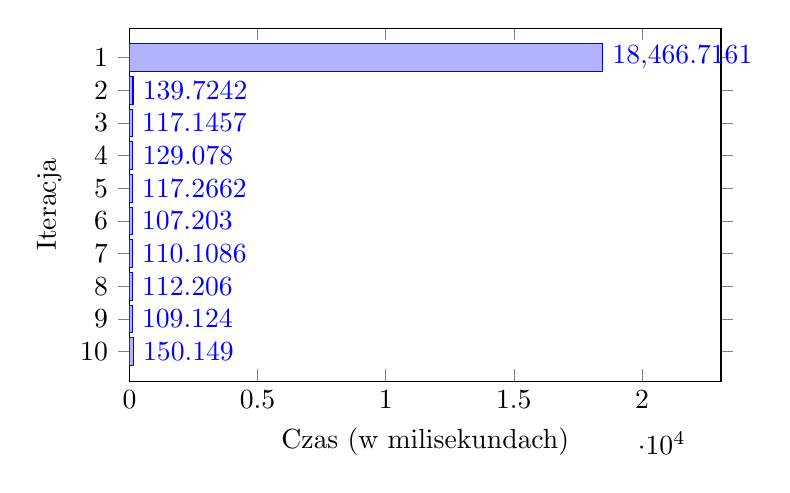
\begin{tikzpicture}
  
    \begin{axis} [
      xbar = .05cm,
      nodes near coords,
      nodes near coords style={
        /pgf/number format/precision=4,
      },
      xmin = 0,
      ytick = data,
      enlarge x limits = {value = .25, upper},
      symbolic y coords = {10,9,8,7,6,5,4,3,2,1},
      xlabel=Czas (w milisekundach),
      ylabel=Iteracja,
      width=0.75\textwidth,
      height=0.5\textwidth
    ]
    
      \addplot coordinates {(18466.716099977493,1) (139.72420001029968,2) (117.1457000374794,3) (129.0780000090599,4) (117.2661999464035,5) (107.2030000090599,6) (110.10860002040863,7) (112.20600003004074,8) (109.1240000128746,9) (150.14899998903275,10)};
      
    \end{axis}
  
  \end{tikzpicture}
  \caption{Wynik testów przykładu 12 [\ref{lst:wydajnosc-przyklad-p-12}]}
  \label{fig:wynik-przyklad-11}
\end{figure}
